\chapter{Ergebnisse}
\section{Einfluss der Auger-Rekombination auf die IQE}
\thispagestyle{fancy}
%
\begin{figure}[ht]
    \centering
    \begin{minipage}[t]{0.49\linewidth}
        \centering
        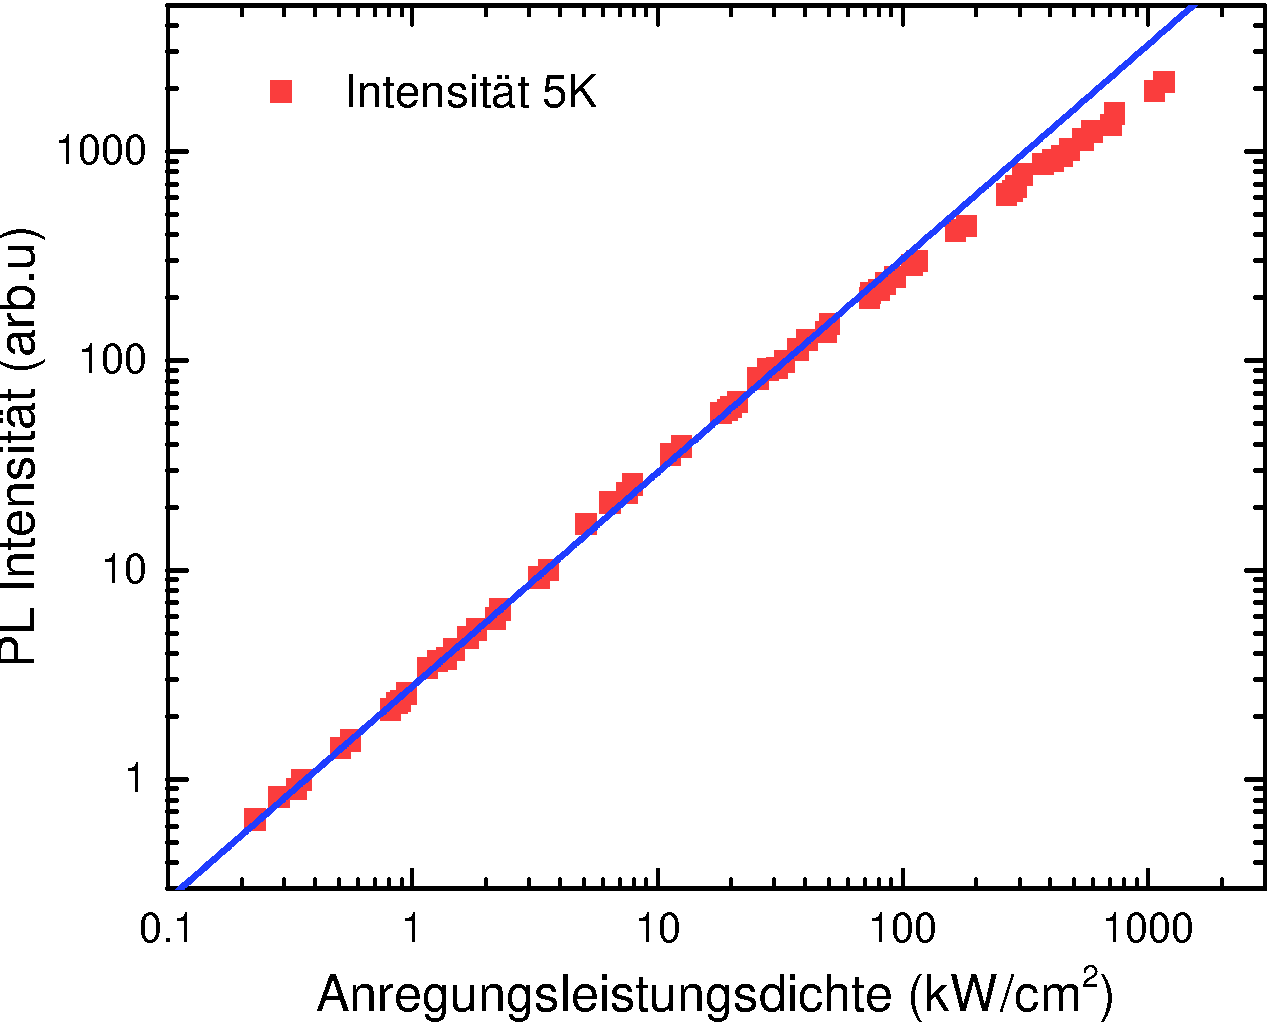
\includegraphics[width=\linewidth]{Bilder/AugerBei5K.pdf}
        \caption{Die Grafik zeigt die integrierte Intensität bei Tieftemperatur ($5 K$) in Abhängigkeit der Anregungsleistungdichte. In doppeltlogarithmischer Darstellung müsste die integrierte Intensität wegen $R = B \cdot n^2$ linear steigen (schwarze Linie).}
        \label{fig:auger5k}
    \end{minipage}% <- sonst wird hier ein Leerzeichen eingefügt
    \hfill
    \begin{minipage}[t]{0.49\linewidth}
        \centering
        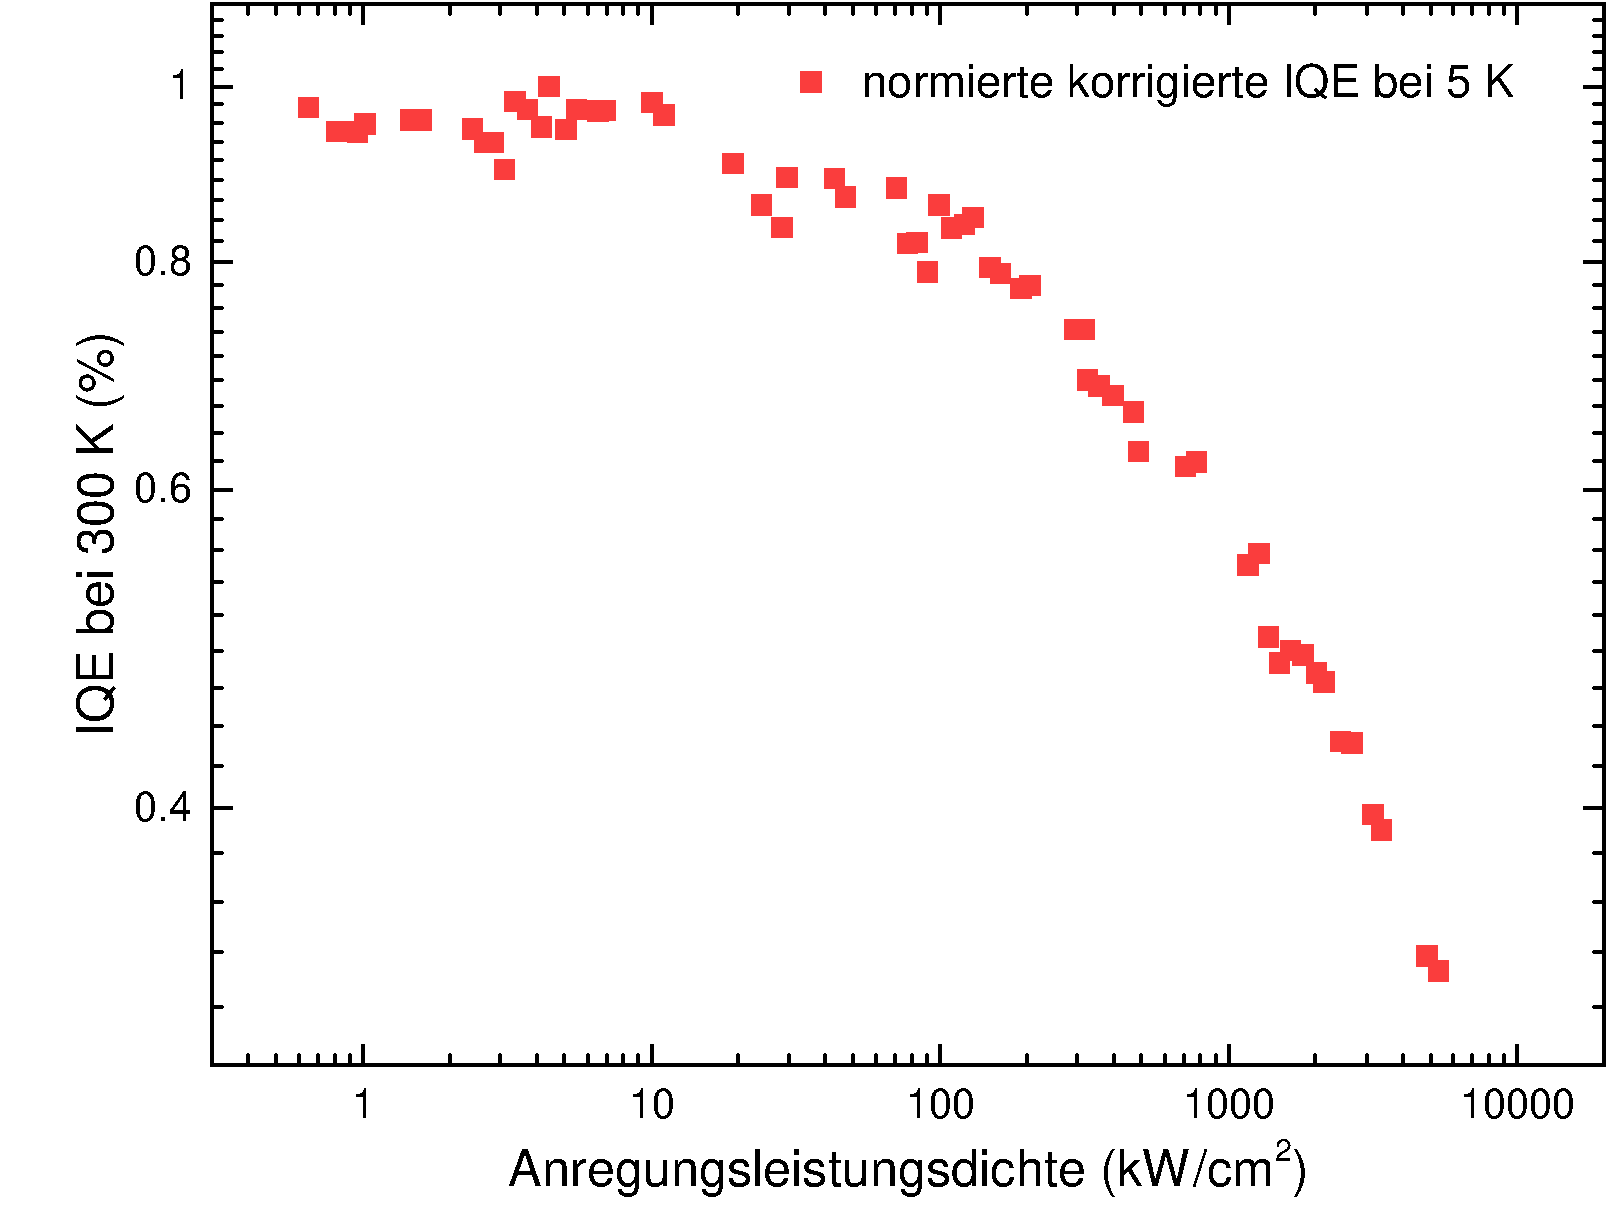
\includegraphics[width=\linewidth]{Bilder/NormierteKorrgierteIQE5K.pdf}
        \caption{Die Grafik zeigt die normierte korrigierte IQE bei 5K nach Gleichung [\ref{eq:iqetrue5k}] }
        \label{fig:trueiqe}
    \end{minipage}
\end{figure}
\vspace{0.1cm}
\raggedright
Das bisher benutzte Modell zur Bestimmung der PL-IQE ging davon aus, dass bei Tieftemperatur keine Auger-Rekombination (Gleichung) vorkommt, aber wie in Abb. [\ref{fig:auger5k}] deutlich zu erkennen, nimmt der Verlauf der PL-Intensität in doppeltlogarithmischer Darstellung gegenüber der Anregungsleistungsdichte (die direkt proportional zur Ladungsträgerdichte ist), im Bereich höherer Anregungsleistungen (entsprechend höheren Ladungsträgerdichten) deutlich ab und weist keinen linearen Verlauf mehr auf, den er aber durch eine allein quadratische Abhängigkeit (in doppeltlogarithmischer Darstellung linear) haben sollte. Dies zeigt, dass die IQE nicht, wie bisher angenommen, immer bei 100 Prozent liegt, sondern auch bei Tieftemperatur Anregungsleistungsdichte abhängig ist. Um dies zu berücksichtigen, wird nun die IQE bei 5K definiert als:
%
\begin{equation}
    IQE_{corr}(T = 5K, P_{exc}) = \frac{ \frac{I_{pl}(T,P_{exc}) }{P_{exc} } } { I_{norm}}
    \label{eq:iqetrue5k}
\end{equation}
%
mit dem Maximum der Verhältnisse von integrierter PL-Intensität zu Anregungsleistungdichte als  Normierungsfaktor über alle $n$ Anregungsleistungdichten
\begin{equation}
    I_{norm} = \lvert \lvert \sum_{i=1}^{n} \frac{I_{pl}(T,P_{exc,i})}{P_{exc,i}} \lvert \lvert_{max}
    \label{eq:iplnorm}
\end{equation}
%
\begin{figure}[tb]
    \centering
    \begin{minipage}[t]{0.49\linewidth}
        \centering
        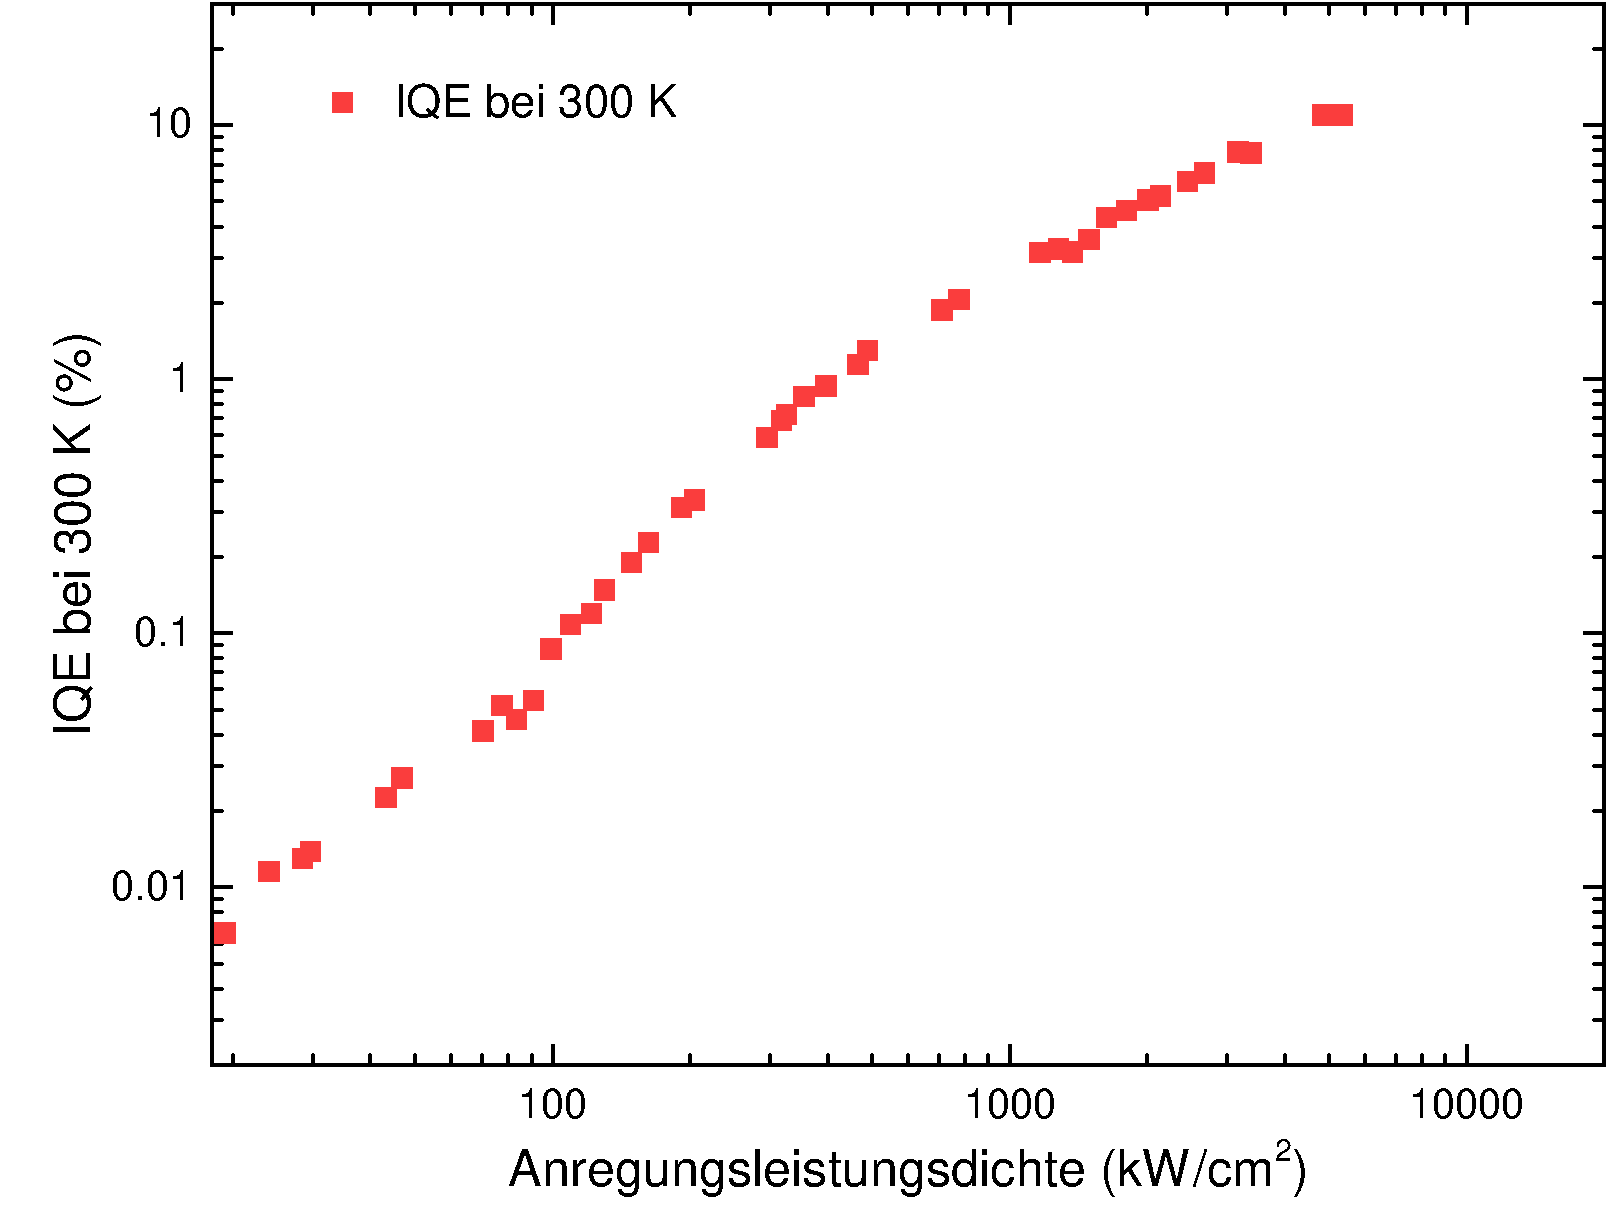
\includegraphics[width=\linewidth]{Bilder/StandardIQE300K.pdf}
        \caption{Die Grafik zeigt die IQE bei Raumtemperatur nach der Methode, die die Auger-Rekombination bei Tieftemperatur als vernachlässigbar betrachtet.}
        \label{fig:standiqe300k}
    \end{minipage}% <- sonst wird hier ein Leerzeichen eingefügt
    \hfill
    \begin{minipage}[t]{0.49\linewidth}
        \centering
        \includegraphics[width=\linewidth]{Bilder/KorrigierteIQE300K.pdf}
        \caption{Die Grafik zeigt die korrigierte IQE bei 300K nach Gleichung [\ref{eq:iqetrue5k}] }
        \label{fig:trueiqe300k}
    \end{minipage}
\end{figure}
\vspace{0.1cm}
\raggedright
%
Wobei $I_{pl}(P_{exc})$ die von der Anrengungsleistungsdichte $P_{exc}$ und Temperatur $T = 5K$ abhängige integrierte PL-Intensität ist. Die integrierte PL-Intensität wird durch die Anregungsleistungsdichte dividiert und auf das Maxmimum normiert, so dass das Maximum der IQE bei $5K$ bei der geringsten Anregungsleistungdichte mit der geringsten Auger-Rekombination liegen sollte. Um nun die IQE bei Raumtemperatur zu bestimmen, wird die nach dem alten Verfahren ermittelte IQE multipliziert mit den neu ermittelten Werten passend zur Anregungsleistungsdichte. 
%
\begin{equation}
    IQE_{corr}(T, A_{exc}) = \frac{IQE(T,A_{exc})}{IQE(5K,A_{exc})} \cdot IQE_{corr}(5K,A_{exc})
    \label{eq:iqetrue300}
\end{equation}
%
Die IQE bei $5K$ dient hierbei also als Skalierungsfaktor, der den Einfluss der Auger-Rekombination bei Raumtemperatur korrigiert. Somit fällt im Vergleich insbesondere auf, dass die Skalierung bei den kleinsten Anregungsleistungsdichten am geringsten Einfluss hat und mit steigender Anregungsleistungsdichte kubisch steigt, so dass die nach dem alten Verfahren ermittelten IQE-Werte bei höheren Anregungsleistungsdichten deutlich nach unten korrigiert werden müssen. 

%
fssfsdf
